Given this, a theory can be categorised purely by the composition law it
exhibits, which is to say by its correction $\epsilon$. What that
correction measures is easiest to see once the recursion is drawn.

\subsection*{The geometry of refinement}
\label{subsec:geometry-of-refinement}
Divide a square into four quadrants and visit them in a fixed order, up
the left-hand side, across the top and down the right-hand side. Divide
each quadrant into four again and visit its sub-squares in the same
pattern, rotated or reflected so that the last sub-square of one
quadrant is adjacent to the first sub-square of the next. After $k$
such steps the path passes once through each of the $4^k$ cells of a
$2^k\times2^k$ grid, moving only between neighbouring cells, as in
Fig.~\ref{fig:refinement-cost-laws}(a). This path is the order-$k$
approximation of the curve introduced by
Hilbert~\cite{hilbert1891stetige}. As $k\to\infty$ it converges to a
continuous curve through every point of the square, the standard
example of a space-filling curve. Cells that are close along the path
are close in space, which is why such curves are used to order data in
spatial databases and large matrix
computations~\cite{haverkort2011inventory}.

\begin{figure*}[t]
  \centering
  \definecolor{fblue}{RGB}{0,114,178}
  \definecolor{forange}{RGB}{230,159,0}
  \definecolor{fdorange}{RGB}{204,121,0}
  \definecolor{fgrey}{RGB}{140,146,152}
  \definecolor{fink}{RGB}{36,48,57}
  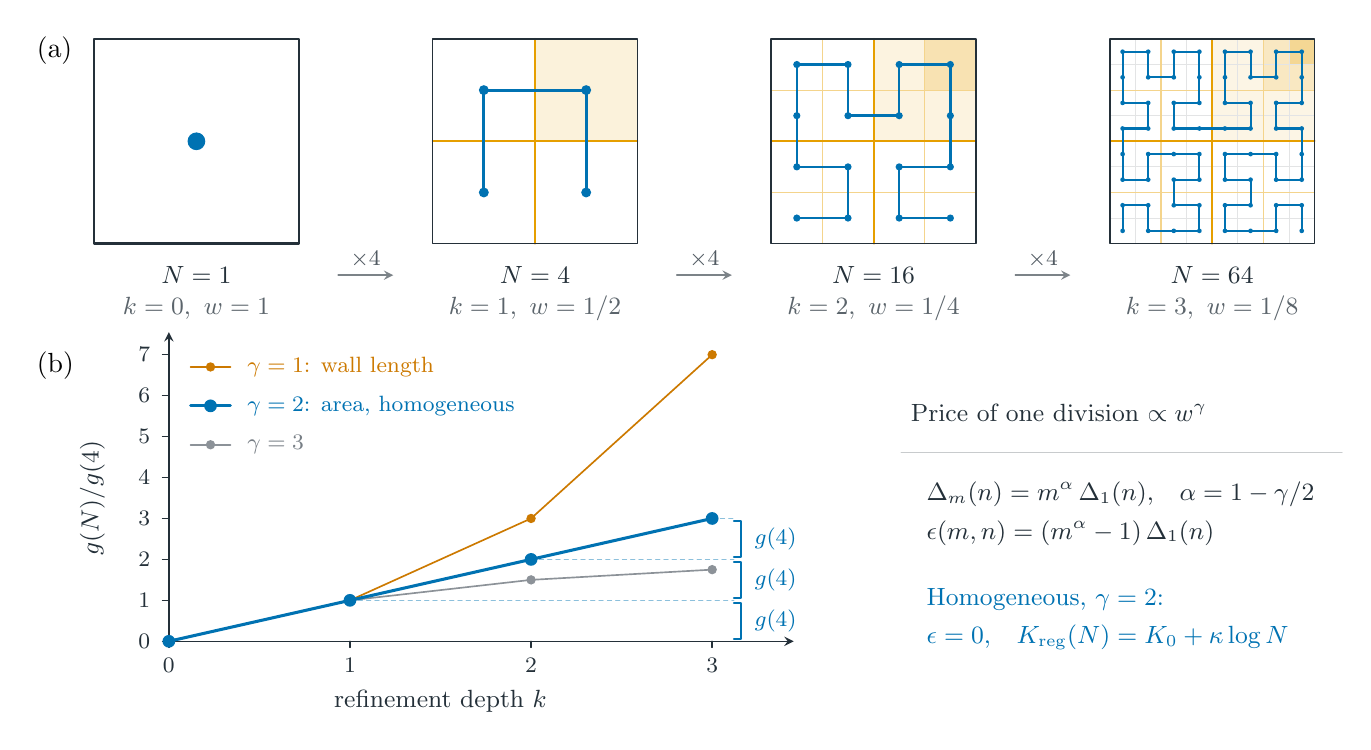
\begin{tikzpicture}[x=1cm,y=1cm,font=\small,line cap=round,line join=round]
  \def\sqside{2.6}
  \node[anchor=north west,font=\normalsize] at (-0.1,8.95) {(a)};
  \begin{scope}[shift={(0.75,6.2)}]
    \draw[fink,line width=0.9pt] (0,0) rectangle (\sqside,\sqside);
    \fill[fblue] (\sqside/2,\sqside/2) circle (3.2pt);
  \end{scope}
  \begin{scope}[shift={(5.05,6.2)},x=1.3cm,y=1.3cm]
    \fill[forange!14] (1,1) rectangle (2,2);
    \draw[forange,line width=0.7pt] (1,0) -- (1,2) (0,1) -- (2,1);
    \draw[fink,line width=0.6pt] (0,0) rectangle (2,2);
    \draw[fblue,line width=1.1pt] plot coordinates {(0.5,0.5) (0.5,1.5) (1.5,1.5) (1.5,0.5)};
    \foreach \i in {0,1} \foreach \j in {0,1} \fill[fblue] (\i+0.5,\j+0.5) circle (1.8pt);
  \end{scope}
  \begin{scope}[shift={(9.35,6.2)},x=0.65cm,y=0.65cm]
    \fill[forange!12] (2,2) rectangle (4,4);
    \fill[forange!30] (3,3) rectangle (4,4);
    \draw[forange!45,line width=0.4pt] (1,0) -- (1,4) (3,0) -- (3,4) (0,1) -- (4,1) (0,3) -- (4,3);
    \draw[forange,line width=0.7pt] (2,0) -- (2,4) (0,2) -- (4,2);
    \draw[fink,line width=0.6pt] (0,0) rectangle (4,4);
    \draw[fblue,line width=0.95pt] plot coordinates {(0.5,0.5) (1.5,0.5) (1.5,1.5) (0.5,1.5) (0.5,2.5) (0.5,3.5) (1.5,3.5) (1.5,2.5) (2.5,2.5) (2.5,3.5) (3.5,3.5) (3.5,2.5) (3.5,1.5) (2.5,1.5) (2.5,0.5) (3.5,0.5)};
    \foreach \i in {0,...,3} \foreach \j in {0,...,3} \fill[fblue] (\i+0.5,\j+0.5) circle (1.3pt);
  \end{scope}
  \begin{scope}[shift={(13.65,6.2)},x=0.325cm,y=0.325cm]
    \fill[forange!10] (4,4) rectangle (8,8);
    \fill[forange!24] (6,6) rectangle (8,8);
    \fill[forange!42] (7,7) rectangle (8,8);
    \draw[fink!13,line width=0.3pt] (1,0) -- (1,8) (3,0) -- (3,8) (5,0) -- (5,8) (7,0) -- (7,8) (0,1) -- (8,1) (0,3) -- (8,3) (0,5) -- (8,5) (0,7) -- (8,7);
    \draw[forange!45,line width=0.4pt] (2,0) -- (2,8) (6,0) -- (6,8) (0,2) -- (8,2) (0,6) -- (8,6);
    \draw[forange,line width=0.7pt] (4,0) -- (4,8) (0,4) -- (8,4);
    \draw[fink,line width=0.6pt] (0,0) rectangle (8,8);
    \draw[fblue,line width=0.75pt] plot coordinates {(0.5,0.5) (0.5,1.5) (1.5,1.5) (1.5,0.5) (2.5,0.5) (3.5,0.5) (3.5,1.5) (2.5,1.5) (2.5,2.5) (3.5,2.5) (3.5,3.5) (2.5,3.5) (1.5,3.5) (1.5,2.5) (0.5,2.5) (0.5,3.5) (0.5,4.5) (1.5,4.5) (1.5,5.5) (0.5,5.5) (0.5,6.5) (0.5,7.5) (1.5,7.5) (1.5,6.5) (2.5,6.5) (2.5,7.5) (3.5,7.5) (3.5,6.5) (3.5,5.5) (2.5,5.5) (2.5,4.5) (3.5,4.5) (4.5,4.5) (5.5,4.5) (5.5,5.5) (4.5,5.5) (4.5,6.5) (4.5,7.5) (5.5,7.5) (5.5,6.5) (6.5,6.5) (6.5,7.5) (7.5,7.5) (7.5,6.5) (7.5,5.5) (6.5,5.5) (6.5,4.5) (7.5,4.5) (7.5,3.5) (7.5,2.5) (6.5,2.5) (6.5,3.5) (5.5,3.5) (4.5,3.5) (4.5,2.5) (5.5,2.5) (5.5,1.5) (4.5,1.5) (4.5,0.5) (5.5,0.5) (6.5,0.5) (6.5,1.5) (7.5,1.5) (7.5,0.5)};
    \foreach \i in {0,...,7} \foreach \j in {0,...,7} \fill[fblue] (\i+0.5,\j+0.5) circle (0.85pt);
  \end{scope}
  \foreach \x/\n/\k/\wl in {0.75/1/0/1,5.05/4/1/{1/2},9.35/16/2/{1/4},13.65/64/3/{1/8}} {
    \node[text=fink] at (\x+1.3,5.8) {$N=\n$};
    \node[text=fink!75] at (\x+1.3,5.38) {$k=\k,\ w=\wl$};
  }
  \foreach \x in {3.35,7.65,11.95} {
    \draw[fink!60,line width=0.5pt,->,>={stealth}] (\x+0.5,5.8) -- (\x+1.2,5.8);
    \node[text=fink!80,font=\footnotesize] at (\x+0.85,6.0) {$\times 4$};
  }
  \node[anchor=north west,font=\normalsize] at (-0.1,4.95) {(b)};
  \begin{scope}[shift={(1.7,1.15)},x=2.3cm,y=0.52cm]
    \draw[fink,line width=0.5pt,->,>={stealth}] (0,0) -- (3.45,0);
    \draw[fink,line width=0.5pt,->,>={stealth}] (0,0) -- (0,7.55);
    \foreach \k in {0,1,2,3} {\draw[fink,line width=0.5pt] (\k,0) -- (\k,-0.15); \node[text=fink,font=\footnotesize,anchor=north] at (\k,-0.18) {$\k$};}
    \foreach \y in {0,...,7} {\draw[fink,line width=0.5pt] (0,\y) -- (-0.035,\y); \node[text=fink,font=\footnotesize,anchor=east] at (-0.05,\y) {$\y$};}
    \node[text=fink,anchor=north] at (1.5,-0.95) {refinement depth $k$};
    \node[text=fink,rotate=90,anchor=south] at (-0.3,3.5) {$g(N)/g(4)$};
    \draw[fgrey,line width=0.6pt] plot coordinates {(0,0) (1,1) (2,1.5) (3,1.75)};
    \foreach \p in {(0,0),(1,1),(2,1.5),(3,1.75)} \fill[fgrey] \p circle (1.7pt);
    \draw[fdorange,line width=0.6pt] plot coordinates {(0,0) (1,1) (2,3) (3,7)};
    \foreach \p in {(0,0),(1,1),(2,3),(3,7)} \fill[fdorange] \p circle (1.7pt);
    \draw[fblue!45,line width=0.4pt,dash pattern=on 1.5pt off 1.5pt] (1,1) -- (3.12,1) (2,2) -- (3.12,2) (3,3) -- (3.12,3);
    \draw[fblue,line width=1.1pt] plot coordinates {(0,0) (1,1) (2,2) (3,3)};
    \foreach \p in {(0,0),(1,1),(2,2),(3,3)} \fill[fblue] \p circle (2.3pt);
    \foreach \y in {0,1,2} {\draw[fblue,line width=0.7pt] (3.12,\y+0.06) -- (3.16,\y+0.06) -- (3.16,\y+0.94) -- (3.12,\y+0.94); \node[text=fblue,font=\footnotesize,anchor=west] at (3.18,\y+0.5) {$g(4)$};}
    \begin{scope}[shift={(0.12,6.7)}]
      \draw[fdorange,line width=0.6pt] (0,0) -- (0.22,0); \fill[fdorange] (0.11,0) circle (1.7pt);
      \node[anchor=west,text=fdorange,font=\footnotesize] at (0.26,0) {$\gamma=1$: wall length};
      \draw[fblue,line width=1.1pt] (0,-0.95) -- (0.22,-0.95); \fill[fblue] (0.11,-0.95) circle (2.3pt);
      \node[anchor=west,text=fblue,font=\footnotesize] at (0.26,-0.95) {$\gamma=2$: area, homogeneous};
      \draw[fgrey,line width=0.6pt] (0,-1.9) -- (0.22,-1.9); \fill[fgrey] (0.11,-1.9) circle (1.7pt);
      \node[anchor=west,text=fgrey!80!fink,font=\footnotesize] at (0.26,-1.9) {$\gamma=3$};
    \end{scope}
  \end{scope}
  \node[anchor=west,text=fink,font=\small] at (11.0,4.05) {Price of one division $\propto w^{\gamma}$};
  \draw[fink!25,line width=0.4pt] (11.0,3.55) -- (16.6,3.55);
  \node[anchor=north west,text=fink,align=left] at (11.2,3.3) {$\Delta_m(n)=m^{\alpha}\,\Delta_1(n)$,\quad $\alpha=1-\gamma/2$\\[3pt] $\epsilon(m,n)=(m^{\alpha}-1)\,\Delta_1(n)$};
  \node[anchor=north west,text=fblue,align=left] at (11.2,1.95) {Homogeneous, $\gamma=2$:\\[3pt] $\epsilon=0$,\quad $K_{\mathrm{reg}}(N)=K_0+\kappa\log N$};
  \end{tikzpicture}
  \caption{\textbf{The composition correction as geometry.}
    \textbf{(a)}~Successive depths $k$ of the Hilbert organisation of a
    square, supporting $N=4^k$ distinctions in registers of width
    $w=2^{-k}$. The blue path visits every cell once in rank order and is
    assembled from four rotated or reflected copies of the path one depth
    coarser. Orange lines mark the divisions made at the first two depths,
    the later one fainter, and grey lines those made at the third. The
    shading follows one register into its sub-registers. Each step to the
    next depth repeats one motif, a cross dividing a register into four,
    in every register at once.
    \textbf{(b)}~Excess budget $g(N)=K_{\mathrm{reg}}(N)-K_0$, normalised
    by the price $g(4)$ of the first division, when dividing a register
    of width $w$ costs in proportion to $w^{\gamma}$,
    Eq.~\eqref{eq:geometric-refinement-price}. A price set by wall length
    ($\gamma=1$) doubles at each depth, a price set by area
    ($\gamma=2$) adds the same increment $g(4)$ at every depth, and a
    price falling faster than area ($\gamma=3$) halves. The correction
    $\epsilon(N,4)$ is the amount by which the step from $N$ to $4N$
    exceeds the first step, so only the area-priced organisation has
    $\epsilon=0$ and $K_{\mathrm{reg}}(N)=K_0+\kappa\log N$.}
  \label{fig:refinement-cost-laws}
\end{figure*}

Number the cells in the order the path visits them, and take this
number as the rank of a symbol. The path finishes each quadrant before
it enters the next, so the first $4^{k-1}$ ranks occupy the first
quadrant, the next $4^{k-1}$ the second, and the same holds inside
every quadrant at every depth. A rank therefore names a quadrant, then
a quadrant within that quadrant, and so on down to a single cell. Every
square in the construction is a register for the cells it contains,
while being itself one of the four symbols of the register above it.
This is the double role of a register made literal. The subdivision of
Eq.~\eqref{eq:register-subdivision} holds at every depth without
reordering a single rank, which is why the sixteen symbols of
Fig.~\ref{fig:register-organisation} could be regrouped along one path.
Refinement is just as uniform. Passing from $4^k$ to $4^{k+1}$
distinctions repeats one motif, a cross dividing a register into four,
in each of the $4^k$ registers at depth $k$.

The path fixes how the distinctions nest. It leaves open the price of
each repetition of the motif, and here the geometry has something to
say, because every repetition acts on a smaller square. At depth $i$
the registers have width $w_i=2^{-i}$, in units of the original square,
and there are $w_i^{-2}=4^i$ of them. Suppose that the price of dividing
a register into four depends only on its width, in proportion to
$w^{\gamma}$. The exponent records the dimension of whatever the
division consumes, with $\gamma=0$ for a fixed charge per division,
$\gamma=1$ for walls drawn across the register and $\gamma=2$ for a
resource spread through its area. Refining from $m=4^k$ to $mn$
distinctions, with $n=4^j$, passes through depths $k$ to $k+j-1$. Since
$4^i w_i^{\gamma}=4^{i\alpha}$ with $\alpha=1-\gamma/2$,
\begin{equation}
  \Delta_m(n)
  =\Delta_1(4)\sum_{i=k}^{k+j-1}4^{i}w_i^{\gamma}
  =m^{\alpha}\,\Delta_1(n),
  \label{eq:geometric-refinement-price}
\end{equation}
and the composition correction of
Eq.~\eqref{eq:composition-correction} follows at once,
\begin{equation}
  \epsilon(m,n)=\bigl(m^{\alpha}-1\bigr)\,\Delta_1(n).
  \label{eq:geometric-correction}
\end{equation}

Equation~\eqref{eq:geometric-correction} is a statement about copies.
Refining $m$ registers draws the motif $m$ times, and each copy is
narrower by a factor $m^{-1/2}$ and so cheaper by $m^{-\gamma/2}$. The
correction $\epsilon$ is what the multiplication of copies leaves over
once their shrinking has been paid for. The two balance at $\gamma=2$,
when dividing a register costs in proportion to its area. The registers
at every depth tile the same square, so the total area being divided
never changes, and neither does the price of dividing it. This is
homogeneous refinement, with $\epsilon=0$. Walls are the natural case
of a smaller exponent. A partition priced by the length of wall it
draws has $\gamma=1$ and $\alpha=1/2$. Its excess budget is
proportional to the total wall length, $2(\sqrt N-1)$ in units of the
side, so each new depth costs twice as much as the last and
$\epsilon>0$. A price falling faster than area gives $\alpha<0$ and
$\epsilon<0$, and divisions become cheaper with depth until arbitrarily
fine distinctions cost almost nothing.
Figure~\ref{fig:refinement-cost-laws}(b) shows the three regimes on the
same organisation.

The square fixes the rate at which its registers narrow, and with it
the balance point. Nothing in the construction requires the quadrants
to fill the square, however, and relaxing this lets the dimension vary
while the order stays fixed. Shrink each quadrant by a factor $1/s$
instead of $1/2$, keep it in its corner, and repeat. The result is a
self-similar set of similarity dimension $d=\log4/\log s$, running from
Hilbert's square at $s=2$ to $d=1$ at $s=4$
(Fig.~\ref{fig:fractional-hilbert}). The cells are visited in the same
order, so every rank and every register is unchanged. For $d<2$ the set
consists of disconnected pieces and no continuous curve can fill it.
The path drawn in the figure only joins consecutive ranks, but the
order is all the register hierarchy uses. Space-filling curves on
connected self-similar sets have been constructed
systematically~\cite{rao2016spacefilling}. Here the set is disconnected
and only the order is carried over. At depth $i$ there are again $4^i$
registers, now of width $w_i=s^{-i}$, so that $4^i=w_i^{-d}$, and the
sum in Eq.~\eqref{eq:geometric-refinement-price} gives the same result
with
\begin{equation}
  \alpha=1-\frac{\gamma}{d}.
  \label{eq:geometric-exponent}
\end{equation}

The correction $\epsilon$ therefore compares two dimensions, that of
the set in which distinctions are drawn and that of whatever pays for
drawing them, and it carries the sign of $d-\gamma$. Homogeneous
refinement is $\gamma=d$, a price of division proportional to the share
of the set's natural measure that the register holds. With the price
fixed, the dimension alone moves the cost law. A division priced by the
length of the cut separating its four parts has $\gamma=1$, which gives
$\alpha=1/2$ on the square and reaches homogeneous refinement as the
set thins to $d=1$. A $d$-dimensional cube divided into $2^d$ parts by
walls has $\gamma=d-1$ and $\alpha=1/d$. On a line the walls are
points, every division costs the same whatever its length, and the
budget grows in proportion to $N$. This is a unary register, with one
physical element per distinction.

\begin{figure*}[t]
  \centering
  \definecolor{fblue}{RGB}{0,114,178}
  \definecolor{forange}{RGB}{230,159,0}
  \definecolor{fverm}{RGB}{213,94,0}
  \definecolor{fink}{RGB}{36,48,57}
  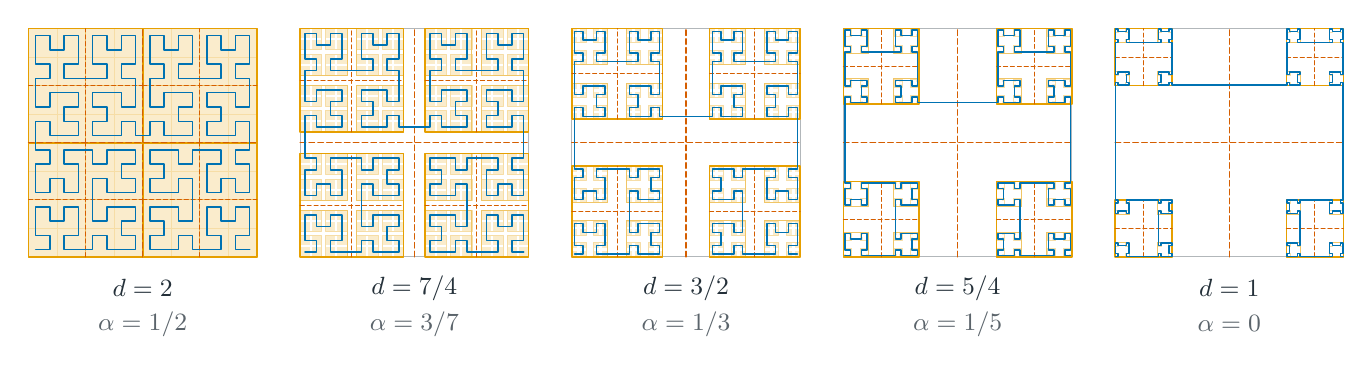
\begin{tikzpicture}[x=1cm,y=1cm,font=\small,line cap=round,line join=round]
  \def\hsq{2.9}
  \def\cpos#1{(\hsq*((1-1/\hs)*(floor((#1)/8)+mod(floor((#1)/4),2)/\hs+mod(floor((#1)/2),2)/(\hs*\hs)+mod((#1),2)/(\hs*\hs*\hs))))}
  \def\cmid#1{(\cpos{#1}+\hsq/(2*\hs*\hs*\hs*\hs))}
  \def\hlist{0/0,0/1,1/1,1/0,2/0,3/0,3/1,2/1,2/2,3/2,3/3,2/3,1/3,1/2,0/2,0/3,0/4,1/4,1/5,0/5,0/6,0/7,1/7,1/6,2/6,2/7,3/7,3/6,3/5,2/5,2/4,3/4,4/4,5/4,5/5,4/5,4/6,4/7,5/7,5/6,6/6,6/7,7/7,7/6,7/5,6/5,6/4,7/4,7/3,7/2,6/2,6/3,5/3,4/3,4/2,5/2,5/1,4/1,4/0,5/0,6/0,6/1,7/1,7/0}
  \foreach \Dval/\Dlab/\alab [count=\p from 0] in {2/{2}/{1/2},1.75/{7/4}/{3/7},1.5/{3/2}/{1/3},1.25/{5/4}/{1/5},1/{1}/{0}} {
   \pgfmathsetmacro\hs{pow(4,1/\Dval)}
   \begin{scope}[shift={(\p*3.45,0)}]
    \draw[fink!35,line width=0.4pt] (0,0) rectangle (\hsq,\hsq);
    \foreach \i in {0,...,15} \foreach \j in {0,...,15} {
      \pgfmathsetmacro\xc{\cpos{\i}}
      \pgfmathsetmacro\yc{\cpos{\j}}
      \fill[forange!20] (\xc,\yc) rectangle ++({\hsq/(\hs*\hs*\hs*\hs)},{\hsq/(\hs*\hs*\hs*\hs)});
    }
    \foreach \i in {0,...,7} \foreach \j in {0,...,7} {
      \pgfmathsetmacro\xb{\hsq*(1-1/\hs)*(floor(\i/4)+mod(floor(\i/2),2)/\hs+mod(\i,2)/(\hs*\hs))}
      \pgfmathsetmacro\yb{\hsq*(1-1/\hs)*(floor(\j/4)+mod(floor(\j/2),2)/\hs+mod(\j,2)/(\hs*\hs))}
      \draw[forange!35,line width=0.25pt] (\xb,\yb) rectangle ++({\hsq/(\hs*\hs*\hs)},{\hsq/(\hs*\hs*\hs)});
    }
    \foreach \i in {0,...,3} \foreach \j in {0,...,3} {
      \pgfmathsetmacro\xb{\hsq*(1-1/\hs)*(floor(\i/2)+mod(\i,2)/\hs)}
      \pgfmathsetmacro\yb{\hsq*(1-1/\hs)*(floor(\j/2)+mod(\j,2)/\hs)}
      \draw[forange!60,line width=0.35pt] (\xb,\yb) rectangle ++({\hsq/(\hs*\hs)},{\hsq/(\hs*\hs)});
    }
    \foreach \i in {0,1} \foreach \j in {0,1} {
      \pgfmathsetmacro\xa{\hsq*(1-1/\hs)*\i}
      \pgfmathsetmacro\ya{\hsq*(1-1/\hs)*\j}
      \draw[forange,line width=0.6pt] (\xa,\ya) rectangle ++({\hsq/\hs},{\hsq/\hs});
    }
    \draw[fverm,line width=0.5pt,dash pattern=on 2pt off 1.2pt] (\hsq/2,0) -- (\hsq/2,\hsq) (0,\hsq/2) -- (\hsq,\hsq/2);
    \foreach \i in {0,1} \foreach \j in {0,1} {
      \pgfmathsetmacro\xa{\hsq*(1-1/\hs)*\i}
      \pgfmathsetmacro\ya{\hsq*(1-1/\hs)*\j}
      \draw[fverm,line width=0.35pt,dash pattern=on 1.5pt off 1pt] ({\xa+\hsq/(2*\hs)},\ya) -- ++(0,{\hsq/\hs}) (\xa,{\ya+\hsq/(2*\hs)}) -- ++({\hsq/\hs},0);
    }
    \draw[fblue,line width=0.55pt] ({\cmid{0}},{\cmid{0}})
      \foreach \i/\j in \hlist { -- ({\cmid{\j}},{\cmid{\i}}) }
      \foreach \i/\j in \hlist { -- ({\cmid{\i}},{\cmid{\j+8}}) }
      \foreach \i/\j in \hlist { -- ({\cmid{\i+8}},{\cmid{\j+8}}) }
      \foreach \i/\j in \hlist { -- ({\cmid{15-\j}},{\cmid{7-\i}}) };
    \node[text=fink] at (\hsq/2,-0.4) {$d=\Dlab$};
    \node[text=fink!75] at (\hsq/2,-0.85) {$\alpha=\alab$};
   \end{scope}
  }
  \end{tikzpicture}
  \caption{\textbf{The Hilbert order at non-integer dimension.} The
    order-four Hilbert sequence of $N=4^4$ ranks placed on the
    self-similar set generated by four corner maps of ratio $1/s$, with
    $s=4^{1/d}$. Orange outlines mark the registers at depths one to
    three, and shaded cells the individual symbols. Dashed lines are the
    cuts that divide the whole set, and each depth-one register, into
    four. Their lengths are proportional to the width of the register
    divided. The ranks and the nesting are the same in every panel, but
    the registers narrow faster as $d$ falls. With each division priced
    by the length of its cut, $\gamma=1$, the exponent $\alpha=1-1/d$ of
    Eq.~\eqref{eq:geometric-exponent} falls from $1/2$ on Hilbert's
    square to zero, homogeneous refinement, at $d=1$. For $d<2$ the set
    is totally disconnected and the blue path is a guide joining
    consecutive ranks rather than part of the set.}
  \label{fig:fractional-hilbert}
\end{figure*}